% =============================================================================
% SECTION 3 — METHOD
% =============================================================================
% Forward references used:
%   Section~\ref{sec:exp:ablation}
%   Section~\ref{sec:method:cot}
%   Appendix~\ref{app:data}                corpus details (Fig. dataset_categories
%                                          and Table dataset)
%   Appendix~\ref{app:algo}                full algorithm details
% =============================================================================

\section{Method}
\label{sec:method}

\subsection{Motivation: Function Calls as Agent-Like Structures}
\label{sec:method:motivation}

Formally, at step $t$ a coding agent maintains a history $h_t$ and samples
an action $a_t \sim \pi(a_t \mid h_t)$; the environment yields an
observation $o_{t+1} \sim p(o_{t+1} \mid h_t, a_t)$; and the agent
continues conditioned on the full trace,
$\pi(\,\cdot \mid h_t, a_t, o_{t+1})$. Under the function-call/agent-step
correspondence introduced in Section~\ref{sec:intro}
(Figure~\ref{fig:teaser}, left), $h_t$ aligns with the pre-call context,
$a_t$ with the call, $o_{t+1}$ with the return, and the continuation with
downstream usage of the returned value.

This correspondence motivates our central design: extract an agentic
conditioning signal from the structure already present in source code via
the fill-in-the-middle (FIM) objective. The correspondence is
\emph{structural} rather than literal---FIM conditions on a given suffix
while agent inference generates one---but training a model to reason
bidirectionally about function-level dependencies should induce a
representation useful when the ``suffix'' is generated rather than
observed. Standard random-span
FIM~\citep{qwencoder, deepseekcoder, starcoder} captures this
structure only incidentally; we instead construct a \emph{function-aware}
variant that selects masking targets based on program structure and
contextual predictability.

\subsection{Data Collection and Decontamination}
\label{sec:method:data}

We curate a corpus of $990$ Python repositories from GitHub. Starting from
$\sim\!2{,}000$ candidates retrieved by combining a star-count threshold
with ten topic queries, we apply manual quality filtering and remove every
repository whose origin overlaps with the source repositories of
SWE-Bench~\citep{swebench} (verified by repository name and any known
fork). To eliminate the possibility of test-time leakage from
training-data commits, we restrict each repository to commits whose
timestamp precedes the earliest base-commit used in SWE-Bench-Verified
and SWE-Bench-Lite. The filtered corpus contains $\approx 78\mathrm{K}$
self-contained Python files ($\approx 33\mathrm{M}$ lines) and yields
roughly $3\mathrm{B}$ training tokens under the Qwen2.5-Coder tokenizer.
Topic-category breakdown, per-property statistics, license inventory, and
commit hashes are reported in Appendix~\ref{app:data}; the full
repository list will be released to support reproduction.

% \subsection{Function-Aware FIM Target Selection}
% \label{sec:method:selection}

% Given the file source of each repository, our pipeline produces a set of
% mask targets together with the corresponding masked file. Each target is
% a single function or a connected group of $2$--$3$ functions; the latter
% variant is studied in Section~\ref{sec:exp:ablation}. The pipeline has four
% stages: dependency-graph construction, complexity scoring, inferability
% scoring, and threshold-based selection. Figure~\ref{fig:pdg_score}
% illustrates the pipeline on a small example; the full single-function
% selection algorithm is given in Appendix~\ref{app:algo:single}.

% % -----------------------------------------------------------------------------
% % Figure: PDG construction and H/I score computation illustration
% % -----------------------------------------------------------------------------
% \begin{figure}[t]
% \centering
% 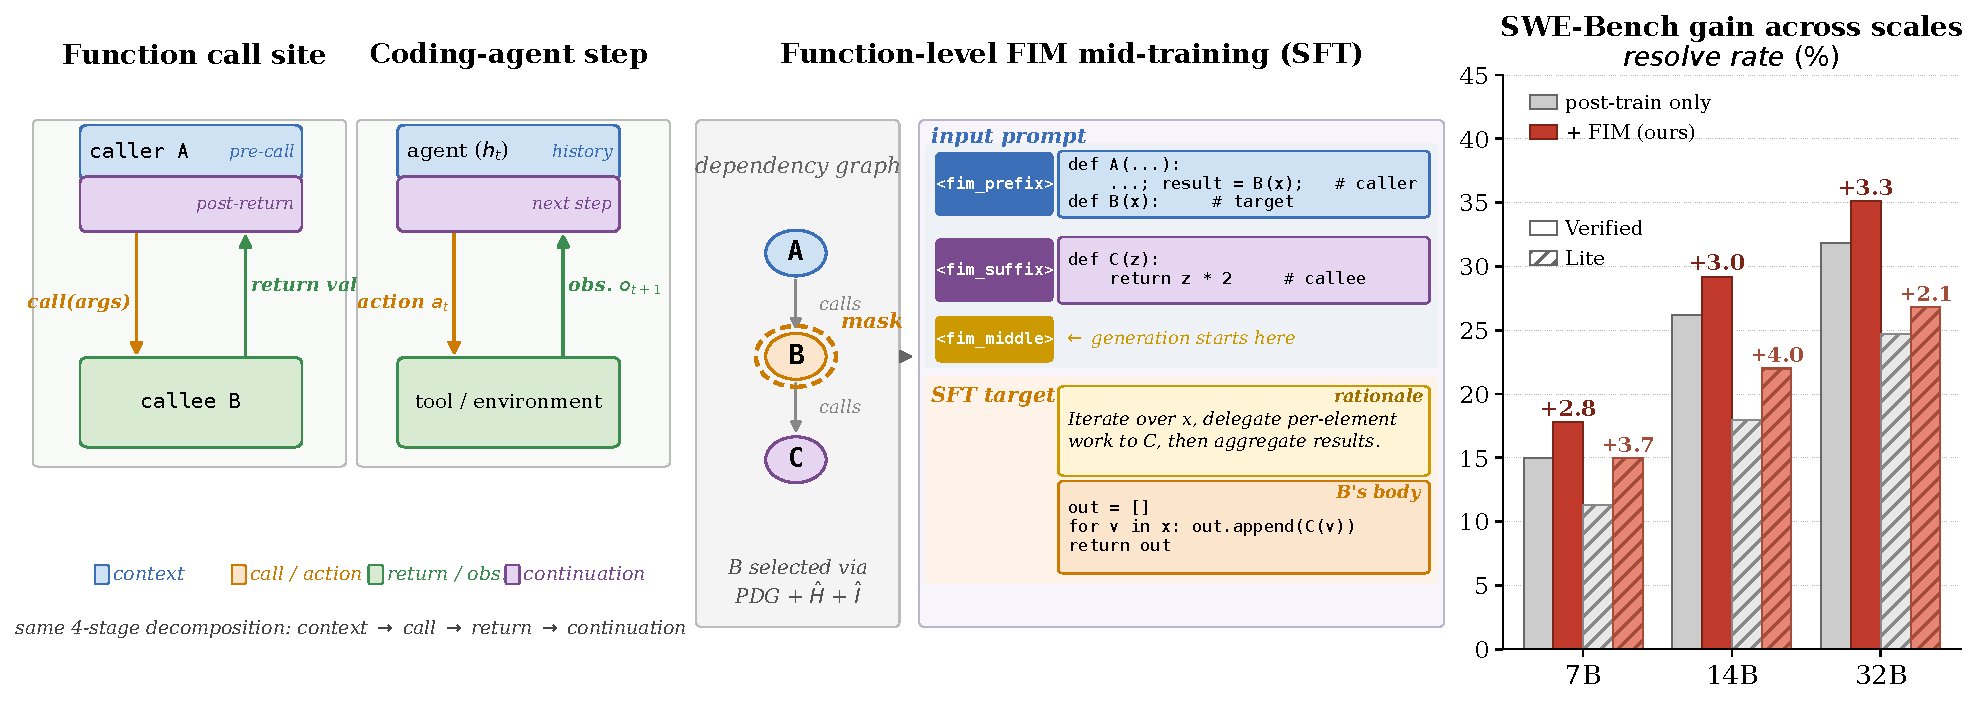
\includegraphics[width=\linewidth]{figs/teaser_v33.pdf}
% \caption{Function-aware FIM target selection on a small example file.
% \textbf{Left:} the program dependency graph (PDG) is constructed by
% parsing the AST: nodes are top-level functions and class methods,
% directed edges $u\!\to\!v$ are call edges in
% $\mathcal{E}_{\mathrm{call}}$, and undirected edges between same-class
% methods are sibling edges in $\mathcal{E}_{\mathrm{sib}}$.
% \textbf{Middle:} for each candidate function $v$ we compute a complexity
% score $\hat{H}(v)$ from lines of code, cyclomatic complexity, and nesting
% depth (Eq.~\ref{eq:complexity}); and an inferability score $\hat{I}(v)$
% that aggregates five context-derived signals (callers, callees,
% signature, docstring, class structure; Eq.~\ref{eq:inferability}).
% \textbf{Right:} the final FIM score combines $\hat{H}$ and $\hat{I}$ via
% a harmonic-mean-like product (Eq.~\ref{eq:fim_single}); functions that
% are simultaneously hard \emph{and} recoverable from context score highest
% and are selected as mask targets.}
% \label{fig:pdg_score}
% \end{figure}

% \subsubsection{Program Dependency Graph}
% \label{sec:method:pdg}

% For each source file we parse its AST and extract the set $\mathcal{V}$
% of function nodes (top-level functions and class methods, identified by
% qualified names). We construct two edge sets: \emph{call edges}
% $\mathcal{E}_{\mathrm{call}}$ between caller and callee, and
% \emph{sibling edges} $\mathcal{E}_{\mathrm{sib}}$ between methods of the
% same class (capturing intra-class coupling that does not manifest as
% direct calls but carries information through shared instance state).
% Call resolution handles common Python idioms (direct invocations, class
% instantiation, \texttt{self}/\texttt{cls} method calls) with a
% short-name fallback against the qualified-name index; details are in
% Appendix~\ref{app:algo:pdg}.

% \subsubsection{Complexity Score $\hat{H}$}
% \label{sec:method:complexity}

% For each $v \in \mathcal{V}$ we define
% %
% \begin{equation}
%   \hat{H}(v) \;=\; w_{\ell}\,\phi\!\left(\mathrm{LoC}(v),\,c_{\ell}\right)
%             + w_{c}\,\phi\!\left(\mathrm{CC}(v),\,c_{c}\right)
%             + w_{d}\,\phi\!\left(\mathrm{D}(v),\,c_{d}\right),
%   \label{eq:complexity}
% \end{equation}
% %
% where $\mathrm{LoC}(v)$ is lines of code, $\mathrm{CC}(v)$ is McCabe
% cyclomatic complexity, $\mathrm{D}(v)$ is the maximum nesting depth of
% control-flow constructs, and $\phi(x, c) = \min(x / c,\, 2)$ normalizes
% each quantity by a soft cap of $2$ (allowing genuinely complex functions
% to score above the median without letting outliers dominate). Caps and
% weights are listed in Appendix~\ref{app:algo:hyperparams}.

% \subsubsection{Inferability Score $\hat{I}$}
% \label{sec:method:inferability}

% A target should be \emph{recoverable} from the surrounding context.
% $\hat{I}(v)$ aggregates five context-derived signals that approximate the
% mutual information between $v$'s body and the rest of the file:
% %
% \begin{equation}
%   \hat{I}(v) \;=\; \alpha\,C_{\mathrm{caller}}(v)
%               + \beta\,C_{\mathrm{callee}}(v)
%               + \gamma\,C_{\mathrm{sig}}(v)
%               + \delta\,C_{\mathrm{doc}}(v)
%               + \varepsilon\,C_{\mathrm{class}}(v).
%   \label{eq:inferability}
% \end{equation}
% %
% $C_{\mathrm{caller}}$ scores call-site argument specificity,
% $C_{\mathrm{callee}}$ counts intra-file functions called by $v$,
% $C_{\mathrm{sig}}$ aggregates type annotations and name descriptiveness,
% $C_{\mathrm{doc}}$ indicates docstring presence, and
% $C_{\mathrm{class}}$ counts in-class siblings; full component formulas
% and weights are in Appendix~\ref{app:algo:inferability}. Each component
% is a hand-designed proxy rather than a learned predictability score: a
% learned proxy would couple selection to a particular reference model and
% complicate the cross-base-model generalization analysis
% (Section~\ref{sec:exp:main}).

% \subsubsection{Single-Function Score}
% \label{sec:method:single}

% The final score combines $\hat{H}$ and $\hat{I}$ in a harmonic-mean-like
% form that requires both to be simultaneously high, multiplied by a
% one-sided difficulty penalty $\rho(\Delta(v))$:
% %
% \begin{equation}
%   \mathrm{FIM}(v) \;=\;
%   \frac{\hat{H}(v)\,\hat{I}(v)}{\hat{H}(v) + \hat{I}(v) + \epsilon}
%   \cdot \rho\!\left(\Delta(v)\right),
%   \label{eq:fim_single}
% \end{equation}
% %
% where $\epsilon$ is a small constant. The harmonic-mean form forces both
% $\hat{H}$ and $\hat{I}$ to be large simultaneously, penalizing imbalance;
% the penalty $\rho$ down-weights targets that remain hard even given full
% context (which would otherwise be unlearnable noise). Full forms of
% $\Delta$ and $\rho$, together with the hard filters on length, dunder
% methods, and minimum scores, are deferred to
% Appendix~\ref{app:algo:penalty}.

% \subsubsection{Multi-Function Group Selection}
% \label{sec:method:groups}

% Real-world code patches frequently span multiple related
% functions~\citep{swebench}, motivating an extension that masks
% \emph{groups} of $k=2$ or $k=3$ structurally connected functions; we use
% this variant only in the granularity ablation
% (Section~\ref{sec:exp:ablation}). A group score $\mathrm{FIM}(G)$
% multiplies a coupling term, the harmonic-mean-like product of
% group-level $\hat{H}(G)$ and $\hat{I}(G)$, and a difficulty penalty,
% with $\hat{I}(G)$ recomputed under joint masking so that intra-group
% references cannot inflate the score. Topology patterns (eight in total:
% caller-callee, co-callee, sibling-coupled, mutual-call, call-chain, hub,
% fan-in, class-triad), the full equations, and selection thresholds are
% given in Appendix~\ref{app:algo:groups}.

% \subsection{Chain-of-Thought Augmentation}
% \label{sec:method:cot}

% For each selected target we generate a natural-language rationale via
% Gemini-3-Preview prompted with the masked file and the original function
% body (template in Appendix~\ref{app:algo:cot}). At training time, the
% rationale is embedded \emph{inside} the FIM middle span, immediately
% before the function body:
% %
% \begin{center}\small
% \texttt{<fim\_prefix>}\,$\langle$prefix$\rangle$\,%
% \texttt{<fim\_suffix>}\,$\langle$suffix$\rangle$\,%
% \texttt{<fim\_middle>}\,$\langle$rationale$\rangle$\,$\langle$body$\rangle$
% \end{center}
% %
% The model is therefore trained to produce, in order, a reasoning trace
% followed by code consistent with that trace---mirroring the
% think-then-act structure of an agent step. The role of the rationale is
% to provide a structured intermediate supervision aligned with the FIM
% objective rather than to distill the teacher's generic capability; we
% isolate this in Section~\ref{sec:exp:ablation} via a \emph{self-CoT}
% variant in which the model under training generates its own rationales,
% and find that the FIM structure alone already accounts for a substantial
% fraction of the gain.


\subsection{Function-Aware FIM Target Selection}
\label{sec:method:selection}

Given the file source of each repository, our pipeline produces a set of
mask targets together with the corresponding masked file. Each target is
a single function or a connected group of $2$--$3$ functions; the latter
variant is studied in Section~\ref{sec:exp:ablation}. The pipeline has
four stages: dependency-graph construction, complexity scoring,
inferability scoring, and threshold-based selection.
Figure~\ref{fig:pdg_score} traces all four stages on a deliberately
small example---a calculator class with two top-level helpers---which we
will use as a running example throughout this subsection. The full
single-function selection algorithm is given in
Appendix~\ref{app:algo:single}; every quantity shown in
Figure~\ref{fig:pdg_score}(b)---including the line-by-line counts
that produce $\mathrm{LoC}\!=\!10$, $\mathrm{CC}\!=\!5$,
$\mathrm{D}\!=\!3$, and the five inferability components---is derived
explicitly in Appendix~\ref{app:algo:worked_example}.

% -----------------------------------------------------------------------------
% Figure: PDG construction and H/I score computation illustration
% -----------------------------------------------------------------------------
\begin{figure}[t]
\centering

\includegraphics[width=\linewidth]{figs/pdg_score.pdf}
% \caption{Function-aware FIM target selection illustrated on a small
% example file (a calculator class with two top-level helpers).
% \textbf{(a)~Program dependency graph.} We parse the AST and instantiate
% one node per top-level function (light cyan) and per class method (light
% green, grouped within a class container). Solid directed edges
% $u\!\to\!v$ are call edges $\mathcal{E}_{\mathrm{call}}$; dashed
% undirected edges between same-class methods are sibling edges
% $\mathcal{E}_{\mathrm{sib}}$ that capture intra-class coupling
% transmitted through shared instance state. Here \texttt{total} calls
% \texttt{is\_int} and \texttt{add}; \texttt{mean} calls \texttt{total};
% all four \texttt{Calculator} methods are connected by sibling edges.
% \textbf{(b)~Complexity and inferability for $\mathtt{Calculator.total}$.}
% The complexity score $\hat{H}$ aggregates lines of code, cyclomatic
% complexity, and nesting depth (Eq.~\ref{eq:complexity}); the
% inferability score $\hat{I}$ aggregates five context signals---callers,
% intra-file callees, signature, docstring, and class
% siblings---weighted by Eq.~\ref{eq:inferability}. Each weight and cap
% is annotated underneath the corresponding formula in italic gray, so
% the bar segments are reproducible: e.g., the LoC contribution is
% $w_{\ell}\!\cdot\!\min(10/50,2)\!=\!0.08$. Stacked bars decompose the
% totals $\hat{H}\!=\!0.40$ and $\hat{I}\!=\!0.48$ into per-component
% contributions; the rose box reports the resulting harmonic-mean-like
% FIM score $\approx\!0.22$ (Eq.~\ref{eq:fim_single}), which exceeds the
% threshold $\tau\!=\!0.20$ and triggers selection.
% \textbf{(c)~Selection in the $(\hat{H},\hat{I})$ plane.} Each function
% is mapped to a point: short helpers (\texttt{add}, \texttt{is\_int},
% \texttt{push}, \texttt{mean}) are removed by the LoC and complexity
% hard filters (gray $\times$); only $\mathtt{Calculator.total}$ falls in
% the rose-shaded region $\mathrm{FIM}\!\geq\!\tau$ and is kept as a mask
% target (red disc). The dashed iso-FIM contours visualize the
% harmonic-mean form: targets must be \emph{both} hard \emph{and}
% recoverable from context---high in only one dimension is insufficient.}
\caption{Function-aware FIM target selection illustrated on a small example file (a calculator class with two top-level helpers).}
\label{fig:pdg_score}
\end{figure}

\subsubsection{Program Dependency Graph}
\label{sec:method:pdg}

For each source file we parse its AST and extract the set $\mathcal{V}$
of function nodes (top-level functions and class methods, identified by
qualified names). We construct two edge sets: \emph{call edges}
$\mathcal{E}_{\mathrm{call}}$ between caller and callee, and
\emph{sibling edges} $\mathcal{E}_{\mathrm{sib}}$ between methods of the
same class (capturing intra-class coupling that does not manifest as
direct calls but carries information through shared instance state).
Call resolution handles common Python idioms (direct invocations, class
instantiation, \texttt{self}/\texttt{cls} method calls) with a
short-name fallback against the qualified-name index; details are in
Appendix~\ref{app:algo:pdg}.
Figure~\ref{fig:pdg_score}(a) shows both edge types on the running
example: \texttt{total} reaches the top-level helpers via
$\mathcal{E}_{\mathrm{call}}$, while $\mathcal{E}_{\mathrm{sib}}$
connects the four \texttt{Calculator} methods that share
\texttt{self.history}.

\subsubsection{Complexity Score $\hat{H}$}
\label{sec:method:complexity}

For each $v \in \mathcal{V}$ we define
%
\begin{equation}
  \hat{H}(v) \;=\; w_{\ell}\,\phi\!\left(\mathrm{LoC}(v),\,c_{\ell}\right)
            + w_{c}\,\phi\!\left(\mathrm{CC}(v),\,c_{c}\right)
            + w_{d}\,\phi\!\left(\mathrm{D}(v),\,c_{d}\right),
  \label{eq:complexity}
\end{equation}
%
where $\mathrm{LoC}(v)$ is lines of code, $\mathrm{CC}(v)$ is McCabe
cyclomatic complexity, $\mathrm{D}(v)$ is the maximum nesting depth of
control-flow constructs, and $\phi(x, c) = \min(x / c,\, 2)$ normalizes
each quantity by a soft cap of $2$ (allowing genuinely complex functions
to score above the median without letting outliers dominate). Caps and
weights are listed in Appendix~\ref{app:algo:hyperparams}. The top bar
of Figure~\ref{fig:pdg_score}(b) shows how the three weighted
components combine into $\hat{H}(\texttt{total})\!=\!0.40$ on the
running example, with the hyperparameter values annotated directly
below the formula and the underlying line/branch counts derived in
Appendix~\ref{app:algo:worked_example}.

\subsubsection{Inferability Score $\hat{I}$}
\label{sec:method:inferability}

A target should be \emph{recoverable} from the surrounding context.
$\hat{I}(v)$ aggregates five context-derived signals that approximate the
mutual information between $v$'s body and the rest of the file:
%
\begin{equation}
  \hat{I}(v) \;=\; \alpha\,C_{\mathrm{caller}}(v)
              + \beta\,C_{\mathrm{callee}}(v)
              + \gamma\,C_{\mathrm{sig}}(v)
              + \delta\,C_{\mathrm{doc}}(v)
              + \varepsilon\,C_{\mathrm{class}}(v).
  \label{eq:inferability}
\end{equation}
%
$C_{\mathrm{caller}}$ scores call-site argument specificity,
$C_{\mathrm{callee}}$ counts intra-file functions called by $v$,
$C_{\mathrm{sig}}$ aggregates type annotations and name descriptiveness,
$C_{\mathrm{doc}}$ indicates docstring presence, and
$C_{\mathrm{class}}$ counts in-class siblings; full component formulas
and weights are in Appendix~\ref{app:algo:inferability}. Each component
is a hand-designed proxy rather than a learned predictability score: a
learned proxy would couple selection to a particular reference model and
complicate the cross-base-model generalization analysis
(Section~\ref{sec:exp:main}). The lower bar of
Figure~\ref{fig:pdg_score}(b) decomposes
$\hat{I}(\texttt{total})\!=\!0.48$ into these five contributions; the
class-context term $\varepsilon\,C_{\mathrm{class}}$ dominates because
\texttt{total} sits among three siblings sharing the same instance
state, while the docstring term contributes the least.
A component-by-component derivation of each of the five terms on the
running example is given in Appendix~\ref{app:algo:worked_example}.

\subsubsection{Single-Function Score}
\label{sec:method:single}

The final score combines $\hat{H}$ and $\hat{I}$ in a harmonic-mean-like
form that requires both to be simultaneously high, multiplied by a
one-sided difficulty penalty $\rho(\Delta(v))$:
%
\begin{equation}
  \mathrm{FIM}(v) \;=\;
  \frac{\hat{H}(v)\,\hat{I}(v)}{\hat{H}(v) + \hat{I}(v) + \epsilon}
  \cdot \rho\!\left(\Delta(v)\right),
  \label{eq:fim_single}
\end{equation}
%
where $\epsilon$ is a small constant. The harmonic-mean form forces both
$\hat{H}$ and $\hat{I}$ to be large simultaneously, penalizing imbalance;
the penalty $\rho$ down-weights targets that remain hard even given full
context (which would otherwise be unlearnable noise). Full forms of
$\Delta$ and $\rho$, together with the hard filters on length, dunder
methods, and minimum scores, are deferred to
Appendix~\ref{app:algo:penalty}.
Figure~\ref{fig:pdg_score}(c) makes the geometry of this rule
explicit: dashed iso-FIM contours bend toward the diagonal, so a
function with high $\hat{H}$ but low $\hat{I}$ (or vice versa) lies far
from the threshold curve. On the running example, the four short
helpers are removed by the hard filters before scoring, and only
$\mathtt{Calculator.total}$, with
$\mathrm{FIM}\!\approx\!0.22\!\geq\!\tau\!=\!0.20$, enters the selected
region.

\subsubsection{Multi-Function Group Selection}
\label{sec:method:groups}

Real-world code patches frequently span multiple related
functions~\citep{swebench}, motivating an extension that masks
\emph{groups} of $k=2$ or $k=3$ structurally connected functions; we use
this variant only in the granularity ablation
(Section~\ref{sec:exp:ablation}). A group score $\mathrm{FIM}(G)$
multiplies a coupling term, the harmonic-mean-like product of
group-level $\hat{H}(G)$ and $\hat{I}(G)$, and a difficulty penalty,
with $\hat{I}(G)$ recomputed under joint masking so that intra-group
references cannot inflate the score. Topology patterns (eight in total:
caller-callee, co-callee, sibling-coupled, mutual-call, call-chain, hub,
fan-in, class-triad), the full equations, and selection thresholds are
given in Appendix~\ref{app:algo:groups}.

\subsection{Chain-of-Thought Augmentation}
\label{sec:method:cot}

For each selected target we generate a natural-language rationale via
Gemini-3-Preview prompted with the masked file and the original function
body (template in Appendix~\ref{app:algo:cot}). At training time, the
rationale is embedded \emph{inside} the FIM middle span, immediately
before the function body:
%
\begin{center}\small
\texttt{<fim\_prefix>}\,$\langle$prefix$\rangle$\,%
\texttt{<fim\_suffix>}\,$\langle$suffix$\rangle$\,%
\texttt{<fim\_middle>}\,$\langle$rationale$\rangle$\,$\langle$body$\rangle$
\end{center}
%
The model is therefore trained to produce, in order, a reasoning trace
followed by code consistent with that trace---mirroring the
think-then-act structure of an agent step. The role of the rationale is
to provide a structured intermediate supervision aligned with the FIM
objective rather than to distill the teacher's generic capability; we
isolate this in Section~\ref{sec:exp:ablation} via a \emph{self-CoT}
variant in which the model under training generates its own rationales,
and find that the FIM structure alone already accounts for a substantial
fraction of the gain.